%\documentclass[a4paper,12pt,twoside]{book}
\documentclass[12pt,times]{report}
\usepackage{mathptmx}%This package supersedes times and mathptm
\usepackage[a4paper,right=2.54cm,left=2.54cm,top=2.54cm,bottom=2.54cm]{geometry}

%%%%paquete para usar citas de diferentes formatos
%%%%%%%%%%%%%%%%%%%%%%%%%%%%%%%%%
%%add al indice
%\usepackage[nottoc,numbib]{tocbibind}
%\usepackage[authoryear,round]{natbib}
\usepackage[utf8]{inputenc}
\usepackage{csquotes}
\usepackage[spanish]{babel}
\usepackage[style=apa ,
%hyperref=auto,
%citestyle=authoryear,
natbib=true,
backend=biber]{biblatex}
\addbibresource{biblio/references.bib}
%\usepackage{biblatex}
%paquete para hiperlinks entre citas e imagenes
%%%%%%%%%%%%%%%%%%%%%%%%%%%%%%%%%
\usepackage[colorlinks=true,
citecolor=blue,
urlcolor=cyan,
bookmarks=true,
linkcolor=blue,
pdftitle={Tesis-nombre-alumno},
pdfauthor={autor nombres}]{hyperref}

\usepackage{amssymb}
\usepackage{graphicx} % for improved inclusion of graphics
%\usepackage{wrapfig} % to include figure with text wrapping around it
\usepackage[margin=10pt,font=small,labelfont=bf]{caption} % for improved layout of figure captions with extra margin, smaller font than text
\usepackage{eucal}
\usepackage[usenames, dvipsnames]{color}
\usepackage[perpage]{footmisc}
%\usepackage[round, sort]{natbib}
\usepackage{ifthen}
\usepackage{multicol} % for pages with multiple text columns, e.g. References
\setlength{\columnsep}{20pt} % space between columns; default 10pt quite narrow
\usepackage[nottoc]{tocbibind} % correct page numbers for bib in TOC, nottoc suppresses an entry for TOC itself
\usepackage{appendix}

%%%----Modificar encabezado y pie de pagina
%%%%%%%%%%%%%%%%%%%%%%%%%%%%%%%%%%%%%%%%%%%%%%%%%%%%%%%%%%%%%%%%%%%%%
\usepackage{fancyhdr} % for better header layout
\newcommand{\changefont}{%
	\fontsize{9pt}{1.5pt}\selectfont
}
\pagestyle{fancy}
\fancyhf{} %% delete default configuration of page
%%\setlength\headheight{15pt}
\fancyhead[L]{\changefont }
\fancyhead[R]{\changefont \leftmark}
%%\fancyfoot[L]{\leftmark}
\fancyfoot[R]{\thepage}

%%%%%%%%%%%%%%%%%%%%%%%%%%%%%5
%%%% Configuracion de los parrafos
%\usepackage{setspace}
%\onehalfspacing
%\linespread{1.25} 
\setlength{\parindent}{0.5in} %%sangria
\setlength{\parskip}{3mm}  %%espacio entre parrafos
\linespread{1.3} %This equals 1.5 linespacing in Word
%%%% nuevo parrafo
%%%%%%%%%%%%%%%%%%%%%%%%%%%%%5
%%%% Centrar valores de una tabla
\usepackage{array}
%%CENTRADO HORIZONTAL
\newcolumntype{P}[1]{>{\centering\arraybackslash}p{#1}}
%%CENTRADO VERTICAL
\newcolumntype{M}[1]{>{\centering\arraybackslash}m{#1}}

%%%%%%%%%%%%%%%%%%%%%%%%%%%%%5
%%%%Paquete para alinear texto
\usepackage{ragged2e}
\usepackage{multirow}
\usepackage{makecell}
\usepackage{rotating}
\usepackage{siunitx} % To align the numbers later on
\usepackage[table,xcdraw]{xcolor}
\usepackage{color, colortbl}
\definecolor{Gray}{gray}{0.9}
\definecolor{orange}{rgb}{1,0.647,0}
\definecolor{turq3}{rgb}{0.54, 0.81, 0.94}
\definecolor{turq}{rgb}{0.63, 0.79, 0.95}
\definecolor{bluejean}{rgb}{0.03, 0.27, 0.49}

%%%%%%%%%%%%%%%%%%%%%%%%%
\usepackage{xparse}
\usepackage{expl3}
%%%%funcion de reemplazar regex
\ExplSyntaxOn
\NewDocumentCommand{\replace}{mmm}
{
	\marian_replace:nnn {#1} {#2} {#3}
}

\tl_new:N \l_marian_input_text_tl
\tl_new:N \l_marian_search_tl
\tl_new:N \l_marian_replace_tl

\cs_new_protected:Npn \marian_replace:nnn #1 #2 #3
{
	\tl_set:Nn \l_marian_input_text_tl { #1 }
	\tl_set:Nn \l_marian_search_tl { #2 }
	\tl_set:Nn \l_marian_replace_tl { #3 }
	\regex_replace_all:nnN { \b\u{l_marian_search_tl}\b } { \u{l_marian_replace_tl} } \l_marian_input_text_tl
	\tl_use:N \l_marian_input_text_tl
}
\ExplSyntaxOff

%%%%%%%%%%%%%%%%%%%%%%%%%%%%%%%%%%%%%%
\usepackage{amsmath}
\numberwithin{equation}{chapter} %%enumerar ecuaciones
\renewcommand{\theequation}{Ecuación \thechapter.\arabic{equation}}   
\usepackage{mathtools, nccmath, cool}
%%%Configuraciones de biblatex

%%%hel
%%%%\citeauthor
\makeatletter

%%%%%%%%%%%%
\DeclareCiteCommand{\citeauthor}
{\boolfalse{citetracker}%
	\boolfalse{pagetracker}%
	\usebibmacro{prenote}}
{\ifciteindex
	{\indexnames{labelname}}
	{}%
	\printtext[bibhyperref]{\printnames{labelname}}}
{\multicitedelim}
{\usebibmacro{postnote}}


\DeclareCiteCommand{\citetitle}
{\boolfalse{citetracker}%
	\boolfalse{pagetracker}%
	\usebibmacro{prenote}}
{\ifciteindex
	{\indexfield{indextitle}}
	{}%
	\printtext[bibhyperref]{\printfield[citetitle]{labeltitle}}}
{\multicitedelim}
{\usebibmacro{postnote}}

\DeclareCiteCommand{\cite}
{\usebibmacro{prenote}}
{\usebibmacro{citeindex}%
	\printtext[bibhyperref]{\usebibmacro{cite}}}
{\multicitedelim}
{\usebibmacro{postnote}}

\DeclareCiteCommand*{\cite}
{\usebibmacro{prenote}}
{\usebibmacro{citeindex}%
	\printtext[bibhyperref]{\usebibmacro{citeyear}}}
{\multicitedelim}
{\usebibmacro{postnote}}

\DeclareCiteCommand{\parencite}[\mkbibparens]
{\usebibmacro{prenote}}
{\usebibmacro{citeindex}%
	\printtext[bibhyperref]{\usebibmacro{cite}}}
{\multicitedelim}
{\usebibmacro{postnote}}

\DeclareCiteCommand*{\parencite}[\mkbibparens]
{\usebibmacro{prenote}}
{\usebibmacro{citeindex}%
	\printtext[bibhyperref]{\usebibmacro{citeyear}}}
{\multicitedelim}
{\usebibmacro{postnote}}

\DeclareCiteCommand{\footcite}[\mkbibfootnote]
{\usebibmacro{prenote}}
{\usebibmacro{citeindex}%
	\printtext[bibhyperref]{ \usebibmacro{cite}}}
{\multicitedelim}
{\usebibmacro{postnote}}

\DeclareCiteCommand{\footcitetext}[\mkbibfootnotetext]
{\usebibmacro{prenote}}
{\usebibmacro{citeindex}%
	\printtext[bibhyperref]{\usebibmacro{cite}}}
{\multicitedelim}
{\usebibmacro{postnote}}

\DeclareCiteCommand{\textcite}
{\boolfalse{cbx:parens}}
{\usebibmacro{citeindex}%
	\printtext[bibhyperref]{\usebibmacro{textcite}}}
{\ifbool{cbx:parens}
	{\bibcloseparen\global\boolfalse{cbx:parens}}
	{}%
	\multicitedelim}
{\usebibmacro{textcite:postnote}}
\makeatother
\makeatletter
\let\abx@macro@citeOrig\abx@macro@cite
\renewbibmacro{cite}{%
	\bibhyperref{%
		\let\bibhyperref\relax\relax%
		\abx@macro@citeOrig%
	}%
}
\let\abx@macro@textciteOrig\abx@macro@textcite
\renewbibmacro{textcite}{%
	\bibhyperref{%
		\let\bibhyperref\relax\relax%
		\abx@macro@textciteOrig%
	}%
}%

\makeatother

%%%%%%%%%%%%%%%%%%%%%%%%%%%%%%%%%%%%%%%%%%%
\begin{document}

\begin{titlepage}

	\begin{center}
		%%%cargar imagen
	    
\includegraphics[width=0.45\textwidth]{images_repo/esanlogomin}
		\vspace*{2cm} \\
		UNIVERSIDAD ESAN \vspace*{1ex} \\
		FACULTAD DE INGENIERÍA \vspace*{1ex} \\
		INGENIERÍA DE TECNOLOGÍAS DE INFORMACIÓN Y SISTEMAS\vspace*{8ex} \\
		\textbf{Implementación de una aplicación de visión por computadora que monitorea el consumo de carbohidratos para la prevención del sindrome metabólico en estudiantes universitarios}
		\vspace*{8ex}\\	
		Trabajo de investigación para el curso de Trabajo de Tesis I 
		\vspace*{8ex} \\	
		Nombre alumno: Marissa Fiorella López Guerrero \\
		Asesor: Marks Calderón		
		\vfill
		
		Lima, \today 
		
	\end{center}
\end{titlepage}
%%cambiar nombres de objetos para el indice y otros
%\renewcommand{\listfigurename}{Índice de Figuras}
\renewcommand{\tablename}{Tabla}
\renewcommand{\listtablename}{Índice de Tablas}

%\thispagestyle{plain}
\begin{center}
	\vspace*{1.5cm}
	{\Large \bfseries  Resumen}
\end{center}
\vspace{0.5cm}


\newline

\textbf{ } 
%\thispagestyle{plain}
\begin{center}
	\vspace*{1.5cm}
	{\Large \bfseries  Abstract}
\end{center}
\vspace{0.5cm}


\newline

\textbf{ } 
%\thispagestyle{plain}
\begin{center}
	\vspace*{1.5cm}
	{\Large }
\end{center}


%\thispagestyle{plain}
\begin{center}
	\vspace*{1.5cm}
	{\Large \bfseries  Agradecimientos}
\end{center}
\vspace{0.5cm}

\newline



% outline
\tableofcontents            % print the table of contents

%: ----------------------- contents ------------------------

\setcounter{secnumdepth}{3} % organisational level that receives a numbers
\setcounter{tocdepth}{3}    % print table of contents for level 3

% levels are: 0 - chapter, 1 - section, 2 - subsection, 3 - subsection


%: ----------------------- list of figures/tables ------------------------

%\listoffigures	% print list of figures

\listoftables  % print list of tables



\chapter{PLANTEAMIENTO DEL PROBLEMA}

Para este trabajo de investigación se abordará como tema principal el síndrome metabólico, el cual aumenta el riesgo de enfermedades como la diabetes tipo 2. Este estudio se enfocará en estudiantes universitarios que a menudo descuidan su salud por sus actividades académicas. Para una propuesta de solución se busca utilizar las herramientas de inteligencia artificial como la visión por computadora y las redes neuronales convolucionales con el objetivo de poder clasificar los carbohidratos de los alimentos para prevenir el síndrome metabólico en la comunidad estudiantil, en especial reducir el riesgo de padecer diabetes tipo 2. 

\section{Descripción de la Realidad Problemática}

El síndrome metabólico se refiere a una condición de salud seria que incrementa la probabilidad de padecer afecciones cardíacas, diabetes, episodios cerebrovasculares y enfermedades vinculadas al acumulamiento de grasa en las arterias (aterosclerosis). Para la revista cubana de Medicina Militar \parencite{vera2022combinaciones} el síndrome metabólico es una enfermedad que se caracteriza por la ocurrencia de patologias metabólicas en un largo plazo, como la diabetes tipo 2. Los  factores de riesgo conocido para el desarrollo del síndrome metabólico comprenden el sobrepeso, hipertensión, la obesidad, la resistencia a la insulina, aspectos genéticos, el avance en la edad y, sobre todo, la mala alimentación desde una edad temprana \parencite{lemieux2020metabolic}.

El síndrome metabólico es conocido también como el Síndrome X y la propuesta para su diagnóstico fue dada por el programa Nacional de Educación sobre el Colesterol-Panel de Tratamiento de Adultos III (NCEPATP III) el cual muestran los límites que una persona debe de cumplir para ser diagnosticada por los criterios del síndrome metabólico, los cuales son: la obesidad abdominal, niveles elevados de triglicéridos, niveles bajos de colesterol HD, hipertensiónarterial y niveles elevados de glucosa en ayunas.Entre estos criterios, la diabetes tipo 2 se muestra como un componente central, debido a la resistencia a la insulina que afecta la disfunción en la regulación del azúcar en sangre, la hipertensión arterial y obesidad abdominal. La diabetes tipo 2 no solo aumenta significativamente el riesgo de desarrollar complicaciones cardiovasculares y otros problemas de salud asociados con el síndrome metabólico, sino que también refuerza la importancia de abordar la resistencia a la insulina como un factor central en la gestión y prevención.  

El riesgo a desarrollar diabetes tipo 2 es de 3 a 5 veces mayor en los pacientes con sindrome metabolico a diferencia que la poblacion general \parencite{dobrowolski2022metabolic}. Sin importar la edad en una persona, el síndrome metabólico puede afectar a un individuo en todas las etapas de la vida, incluyendo a jóvenes universitarios. Dentro del ámbito de la vida académica de un estudiante universitario, es usual que su estilo de vida tienda a subestimar la importancia de la salud metabólica. Esto suele ocurrir como consecuencia de la dedicación a los estudios y la presión académica, lo que incrementa el riesgo de desarrollar alguno de los factores de síndrome metabólico, tales como la obesidad, hipertensión y diabetes. Por lo tanto, es importante que logren comprender la importancia de incorporar una alimentación adecuada en su estilo de vida, ello con el fin de poder garantizar un futuro más saludable. Para ello el poder reconocer la importancia de identificar qué alimentos son adecuados para prevenir el síndrome metabólico mediante su clasificación es fundamental. Sin embargo, la realidad es que la mayoría de estudiantes universitarios no cuentan con el conocimiento necesario para llevar un buen seguimiento de su alimentación. 

En este sentido, gracias a los avances tecnológicos, existen herramientas de inteligencia artificial como la visión por computadora y las redes neuronales convolucionales que cumplen un papel importante en ello. La visión por computadora, a través de los descriptores, ayuda a clasificar y evaluar de forma rápida las características de interés de los alimentos. Tambien para este caso y prevenir el síndrome metabólico, nos centraremos en el contenido de carbohidratos de un alimento. En otra palabras, se calculará el contenido de glucosa a partir de los carbohidratos de la tabla nutricional y el indice glucemico.

Para el onsejo Argentino sobre Seguridad de Alimentos y Nutricion \parencite{CISAN} , el indice glucemico es un metodo que mide y clasifica los alimentos que tienen carbohidratos que elevan la glucosa en la sangre una vez consumidos. 

La Organización de las Naciones Unidas para la Alimentación y la Agricultura (FAO) define lo define como  la subida bajo la curva respuesta glucemica que produce al ingerir 50 gramos de hidratos de carbono  o carbohidratos. Existen alimentos que tienen poca o nada de carbohidratos como los huevos y vegetales de hojas verdes. Aunque el indice glucemico tiene alguna limitaciones como el no considerar la respuesta insulínica.

Como indica \parencite{albornoz2012nutricion} , los componentes de la dieta y el sindrome meabólico puede relacionarse con contenidos bajos en carbohidratos y ello puede controlar la insulina, el peso y presion arterial. También menciona que, es importante el tipo de hidrato de carbono o carbohidrato que compone una dieta. 

Lo que facilita la toma de decisiones sobre dietas especializadas y la prevención del síndrome metabólico. De igual manera, las redes neuronales convolucionales o CNN, la cual es adecuada para la tarea de reconocer y clasificar imágenes en función a patrones. No obstante, el uso de descriptores de características de visión por computadora y las redes neuronales convolucionales para la clasificación de componentes alimenticios en la prevención del síndrome metabólico es un área de trabajo que sigue en constante evaluación y desarrollo, es bajo este contexto que se trabajara la presente investigación, buscando clasificar de manera eficiente y certera los componentes alimenticios que puedan reducir el riesgo de que un joven universitario padezca del síndrome metabólico mediante el uso de descriptores de características de visión por computadora y CNN para mejorar su calidad de vida a largo plazo.


\section{Formulación del Problema}

Para la formulación del problema se tomará un problema general el cual plantea la posibilidad de calificar los componentes alimenticios mediante el uso de la inteligencia artificial con el fin de prevenir el síndrome metabólico de la diabetes tipo 2 , obesidad, presion arterial, entre otros usando como base los carbohdratos ingeridos. Los cuales incluyen la búsqueda de una base de datos, la identificación de descriptores efectivos y una búsqueda a la mejor arquitectura de CNN para entrenar un modelo de evaluación de alimentos para una buena salud. Adicionalemnte, la Matriz de consistencia (Anexo 1). 

\subsection{Problema General}
\newcommand{\ProblemaGeneral}{
	¿Es posible crear una aplicación para monitorear carbohidratos aplicando vision por computadora para prevenir el síndrome metabólico en estudiantes universitarios?
}
\ProblemaGeneral
\subsection{Problemas Espec\'{i}ficos}
\newcommand{\Pbone}{
¿Existirá alguna base de datos de imágenes de alimentos etiquetados con su contenido de carbohidratos para poder entrenar un modelo que ayude a prevenir el síndrome metabólico?
}
\newcommand{\Pbtwo}{
¿Cómo medir la efectividad de la aplicación de visión por computadora que monitorea los carbohidratos para ayudar a prevenir el síndrome metabólico en estudiantes universitarios?
}
\newcommand{\Pbthree}{
¿Cuál es la mejor arquitectura de redes neuronales convolucionales (CNN) para poder entrenar un modelo de monitoreo de carbohidratos?
}
\newcommand{\Pbfour}{
¿Cuál es el método de preprocesamiento más adecuado para mejorar la calidad de las imágenes de alimentos para el monitoreo de carbohidratos que presentan un alto nivel de ruido?
}

\begin{itemize}
	\item \Pbone
	\item \Pbtwo
	\item \Pbthree
 	\item \Pbfour
\end{itemize}

\section{Objetivos de la Investigación}

Para la formulación del objetivo se tomará un objetivo general el cual plantea desarrollar una herramienta capaz de clasificar los componentes alimenticios y prevenga los riesgos asociados al  síndrome metabólico a travez de la medicin de carbohidratos. También se mostrarán tres objetivos específicos, los cuales están relacionados con los problemas específicos propuestos anteriormente. 

\subsection{Objetivo General}
\newcommand{\ObjetivoGeneral}{
Desarrollar una aplicacion que monitorée carbohidratos para ayudar a prevenir enfermedades asociadas con el síndrome metabólico en estudiantes universitarios aplicando vision por computadora.
}
\ObjetivoGeneral
\subsection{Objetivos Espec\'{i}ficos}
\newcommand{\Objone}{
Encontrar y/o construir una base de datos de imágenes de alimentos etiquetados con su contenido de carbohidratos para el entrenamiento de un modelo que ayude a prevenir el síndrome metabólico.

}
\newcommand{\Objtwo}{
Determinar la efectividad de la aplicacion que ayuda a prevenir el síndrome metabólico en estudiantes universitarios monitoreando los carbohidratos a traves de vision por computadora 
}
\newcommand{\Objthree}{
Determinar la mejor arquitectura de redes neuronales convolucionales (CNN) para entrenar un modelo de monitoreo de carbohidratos.
}
\newcommand{\Objfour}{
Determinar la mejor arquitectura de redes neuronales convolucionales (CNN) para entrenar un modelo de monitoreo de carbohidratos.
}

\begin{itemize}
	\item {\Objone}
	\item {\Objtwo}
	\item {\Objthree}
	\item {\Objfour} 
\end{itemize}

\section{Hipotesis}

Para la formulación de la hipótesis se tomará una hipótesis general la cual menciona si clasificar los componentes alimenticios ayuda a prevenir los riesgos de síndrome metabólico y tres hipótesis especificas las cuales están relacionadas con la formulación del problema y objetivos específicos.

\subsection{Hipotesis General}
\newcommand{\HipotesisGeneral}{
Crear una aplicación que monitoree carbohidratos mediante visión por computadora ayuda a prevenir los riesgos asociados con el síndrome metabólico en los estudiantes universitarios}
\HipotesisGeneral
\subsection{Hipotesis Específicas}
\newcommand{\Hone}{
 Una base de datos de imágenes de alimentos etiquetados con su contenido de carbohidratos permite entrenar un modelo que ayude a prevenir el síndrome metabólico.
}
\newcommand{\Htwo}{
La efectividad de la aplicacion de visión por computadora que monitorea los carbohidratos ayuda a prevenir el síndrome metabólico en estudiantes universitarios
}
\newcommand{\Hthree}{
La mejor arquitectura de redes neuronales convolucionales (CNN) permite entrenar un modelo de monitoreo de carbohidratos
}
\newcommand{\Hfour}{
 Mediante la aplicación de técnicas de preprocesamiento de imágenes, se logra mejorar la precisión del modelo de monitoreo de carbohidratos al reducir la interferencia del ruido en las imágenes de alimentos.
}


\begin{itemize}
	\item \Hone
	\item \Htwo
	\item \Hthree
 	\item \Hfour
\end{itemize}

\section{Justificación de la Investigación}

Para la justificación de la investigación se tomarán tres puntos principales los cuales mencionan sobre la importancia de medir y consumir alimenticios saludables para poder prevenir el síndrome metabólico utilizando herramientas de inteligencia artificial, mostrando resultados que beneficiarán no solo a la comunidad universitaria sino también a trabajadores y niños en desarrollo.

\subsection{Teórica}

Esta investigación se realiza con el propósito de aportar conocimiento sobre la importancia de adoptar hábitos alimenticios saludables para prevenir los riesgos asociados con el síndrome metabólico en jóvenes universitarios de ESAN. Por ello se emplearán técnicas de inteligencia artificial, como como los descriptores de visión por computadora y las redes neuronales convolucionales (CNN), con el fin de clasificar si un alimento de consumo humano tiene un impacto positivo o negativo en la salud. Los resultados de este estudio no solo beneficiarán a los jóvenes universitarios, sino que también podrán ser aplicados a personas en el ámbito laboral y niños en edad escolar que presentan patrones alimenticios deficientes.

\subsection{Práctica}

Al culminar la investigación se tendrá desarrollada una herramienta que permitirá a cualquier joven universitario mejorar sus hábitos alimenticios para prevenir el síndrome metabólico mejorando así su salud a largo plazo.

\subsection{Metodológica}. 

La implementación de un algoritmo de clasificación de componentes alimenticios promoverá la concientización de la importancia de la alimentación, gracias a que se tendrá más conocimiento de cómo prevenir el síndrome metabólico. Asimismo, permitirá una evaluación más precisa de los alimentos consumidos por los jóvenes universitarios y su relación con los factores de riesgo del síndrome metabólico. A través de la aplicación de inteligencia artificial, se establecerá una metodología sólida para identificar patrones nutricionales y brindar información valiosa que fomente la adopción de hábitos alimenticios más saludables, contribuyendo a la prevención de esta afección y promoviendo el bienestar en la comunidad universitaria.

\section{Delimitación del Estudio}

Esta investigación se centrará en la clasificación de los componentes alimenticios para la prevención del síndrome metabólico en los estudiantes de la universidad ESAN, haciendo uso de descriptores de características de visión por computadora y redes neuronales convolucionales. Para los resultados de la investigación, se espera que en un futuro más personas estén interesadas en cuidar su salud a largo plazo a través del consumo de alimentos para reducir alguno de los cinco criterios de riesgo asociados con el síndrome metabólico.

\subsection{Espacial}
Para la presente investigación se harán pruebas en estudiantes de la universidad ESAN

\subsection{Temporal}
Los datos que serán necesarios para probar el buen uso de la aplicacion abarcara el año 2024

\subsection{Conceptual}
Esta investigación se centrará exclusivamente en la clasificación de componentes alimenticios para la prevención del síndrome metabólico midiendolo a travez de carbohidratos, utilizando descriptores de características de visión por computadora y redes neuronales convolucionales.



\chapter{MARCO TEÓRICO}

En esta sección se abordará los antecedentes de la investigacion relacionadas con herramientas de inteligencia artificial como la visión por computadora, también se incluirán las metodologías y resultados por cada artículo. Adicional, las bases teoricas y el marco conceptual. 


\section{Antecedentes de la investigación}

Los siguientes antecedentes incluyen el resumen, la metodogía y los resultados de papers de revistas y páginas importantes como National Institutes of Health (NIH) y IEEE Xplore Digital Library 

\subsection{Paper 1: A review on vision-based analysis for automatic dietary assessment (2022)}

Los autores son Wang, W., Min, W., Li, T., Dong, X. \& Li, H. de la universidades de Beijing en diferentes carreras, \parencite{wang2022review}

\textbf{Resumen}

\thinspace
Tener una dieta saludable evita problemas de salud a largo plazo, pero algunos métodos para su evaluación suelen ser poco confiables, esto a ido cambiando con la ayuda de la inteligencia artificial, este artículo presenta una arquitectura de Evaluación Dietética Basada en Visión (VBDA) que toma imágenes de una comida como entrada para luego usar visión por computadora e identificar automáticamente información dietética relevante como salida. También se evalúa la arquitectura de múltiples etapas y la de extremo a extremo. Donde la primera, arquitectura de múltiples etapas, consta de tres 3 etapas (análisis de imágenes de alimentos, estimación de volumen y derivación de nutrientes)

\textbf{Metodología}

\thinspace
La arquitectura de múltiples etapas para la Evaluación Dietética Basada en Visión (VBDA) consta de tres fases: análisis de imágenes de alimentos, estimación de porciones y derivación de nutrientes. En el caso del rendimiento de las dos primeras etapas depende de los algoritmos de IA y de los conjuntos de datos, mientras que la última, de base de datos de composición nutricional, como se muestra en la figura \ref{fig1}


\begin{figure}[h]
		\begin{center}
			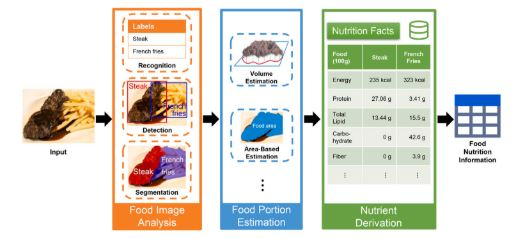
\includegraphics[width=0.8\textwidth]{2/imagen2/6FIGURA6PAPER2.JPG}
			\caption{Arquitectura de múltiples etapas}
			\label{fig1}
		\end{center}
		
	\end{figure}

\thinspace

El análisis de imágenes implica el reconocimiento, detección y segmentación de alimentos, donde el reconocimiento predice el tipo de alimento, la detección localiza y clasifica cada alimento mediante cuadros delimitadores, y la segmentación asigna etiquetas de alimentos a nivel de píxel, proporcionando una localización más precisa para la estimación de porciones, como muestra la figura \ref{fig2}

\begin{figure}[h]
		\begin{center}
			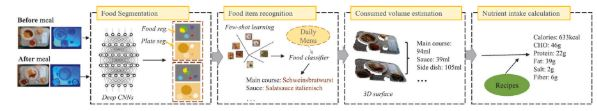
\includegraphics[width=0.8\textwidth]{2/imagen2/8FIGURA8PAPER2.JPG}
			\caption{Evaluación dietética en múltiples etapas}
			\label{fig2}
		\end{center}
		
	\end{figure}

\thinspace

En la arquitectura de extremo a extremo para la Evaluación Dietética Basada en Visión (VBDA) reemplaza múltiples etapas prácticas con una única red neuronal, reduciendo así la propagación y acumulación de errores, mejorando así la precisión y simplificando la optimización conjunta, evitando la necesidad de definir y optimizar etapas separadas con sus respectivas entradas y salidas. Además, de basarse en datos como el volumen de los alimentos, y adopta un marco multitarea para la estimación de nutrientes, abarcando componentes como proteínas y grasas, como se muestra en la figura \ref{fig3}
 
\begin{figure}[h]
		\begin{center}
			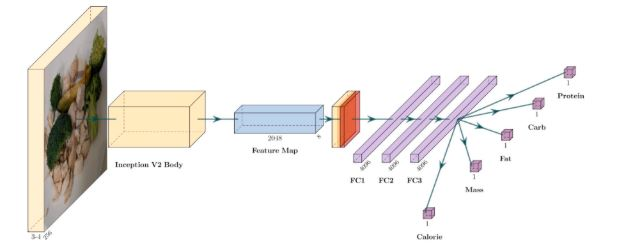
\includegraphics[width=0.8\textwidth]{2/imagen2/7FIGURA7PAPER2.JPG}
			\caption{Evaluación dietética de extremo a extremo}
			\label{fig3}
		\end{center}
		
	\end{figure}

\thinspace
También se usaron métodos para la detección de alimentos en la evaluación dietética implica la localización y reconocimiento de varios alimentos, utilizando técnicas avanzadas como Faster R-CNN y Mask R-CNN para mejorar la eficiencia y precisión del modelo. Estos métodos permiten reducir el área de reconocimiento y manejar propuestas regionales de manera más efectiva, facilitando la estimación de porciones y nutrientes. 

\thinspace

\textbf{Resultados y conclusiones}

\thinspace
La precisión del análisis visual y la estimación del volumen afecta significativamente la precisión de los resultados. En la estimación de volumen, el desempeño de la porción actual de estimación del volumen aún no es satisfactorio y obtener anotaciones precisas de las porciones y la nutrición es costoso por lo que se limita la escala de los conjuntos de datos de VBDA. Aun con ello con los datos recolectados se obtuvo un MAE de 0,0933 sobre estimación de calorías, un chi-cuadrado de 0,73 en estimación de proteínas, en el caso de reconocimiento. 

\subsection{Paper 2: A Comprehensive Survey of Image-Based Food Recognition and Volume Estimation Methods for Dietary Assessment (2021)}

Los autores son Tahir, G. \& Loo, C. del departamento de Inteligencia Artificial, Facultad de Ciencias de la Computación y Tecnología de la Información, Universidad de Malaya, Kuala Lumpur. \parencite{tahir2021comprehensive}

\textbf{Resumen}

\thinspace
Problemas como la obesidad, la hipertensión y diabetes tipo 2 se deben principalmente a una mala alimentación y estilo de vida, aunque existen aplicaciones que te ayuden con ello, suelen ser complicados ya que presentan impresiones por multidimensional, la ambigüedad entre las clases por problemas de reconocimiento de los diferentes alimentos que pueden parecer similares, también están los alimentos ocultos y la calidad de cámara, dando como resultados un bajo rendimiento de los modelos para su reconocimiento. Este artículo muestra las metodologías más efectivas para el reconocimiento de alimentos y su volumen utilizando variantes de redes neuronales convolucionales (CNN) de diferentes artículos. Como el mejorar las representaciones de imágenes de alimentos se utilizan características como la forma, color, textura como métodos visuales, también reducen la complejidad eliminando características redundantes y para el volumen el proceso en su mayoría implica de dos pasos, múltiples imágenes o una sola imagen de una cámara móvil y el cálculo del volumen de alimentos a partir de una construcción 3D o un objeto de calibración. El alcance y taxonomía de este estudio se muestra el gráfico de la figura \ref{fig4}

\begin{figure}[h]
		\begin{center}
			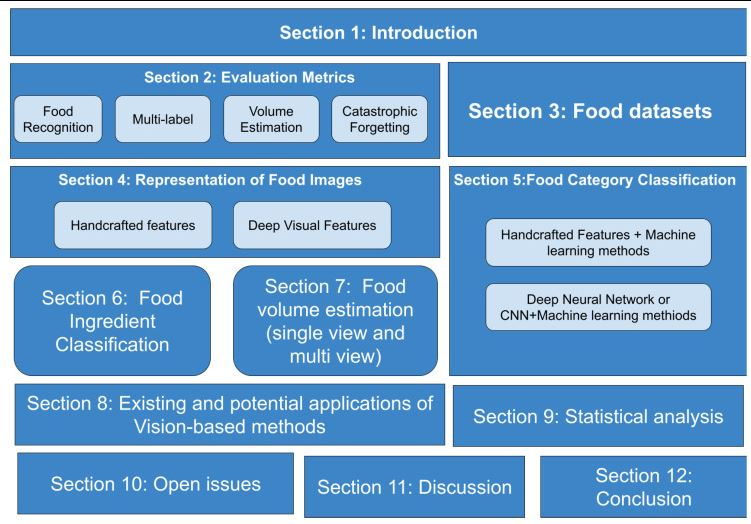
\includegraphics[width=0.6\textwidth]{2/imagen2/1FIGURA1PAPER1.JPG}
			\caption{Alcance de este estudio}
			\label{fig4}
		\end{center}
		
	\end{figure}

\thinspace
\textbf{Metodología}

\thinspace
Para la categorización de alimentos en su mayoría de artículos revisados se utilizaron métricas de evaluación como la matriz de confusión, Exactitud, Precisión, Recall, F1 Score. Para la representación de imágenes de alimentos se utilizaron principalmente dos métodos Handcrafted Features y Deep Visual Feature. En Handcrafted Features se extraen propiedades de las imágenes por algoritmos diseñados manualmente con el fin de capturar información relevante como la textura, forma y color de los alimentos, como lo muestra la figura \ref{fig5}. En Deep Visual Features, se usaron los siguiente clasificadores para el reconocimiento de imágenes de alimentos: máquinas de vectores de soporte (SVM), aprendizaje de núcleo múltiple (MKL) y K-vecino más cercano (KNN).

\begin{figure}[h]
		\begin{center}
			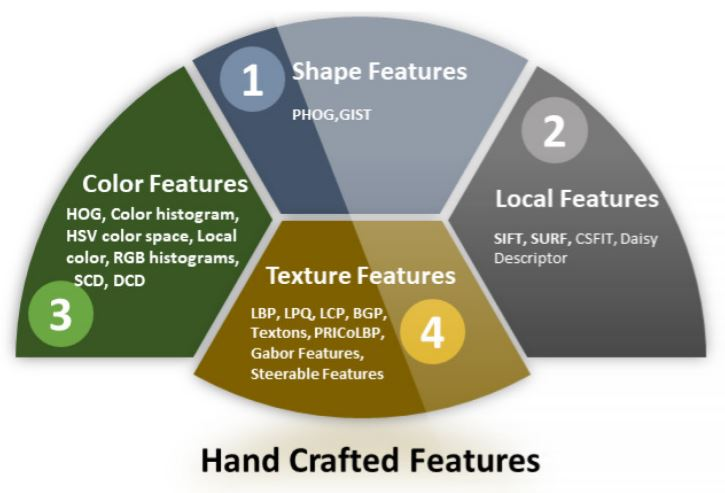
\includegraphics[width=0.7\textwidth]{2/imagen2/2FIGURA2PAPER1.JPG}
			\caption{métodos de extracción: Handcrafted feature}
			\label{fig5}
		\end{center}
		
	\end{figure}

\thinspace

Para la estimación del volumen de alimentos se categoriza como método de “vista de una sola imagen” y de “vista de múltiples imágenes/vídeo”, como muestra la figura \ref{fig6}

\begin{figure}[h]
		\begin{center}
			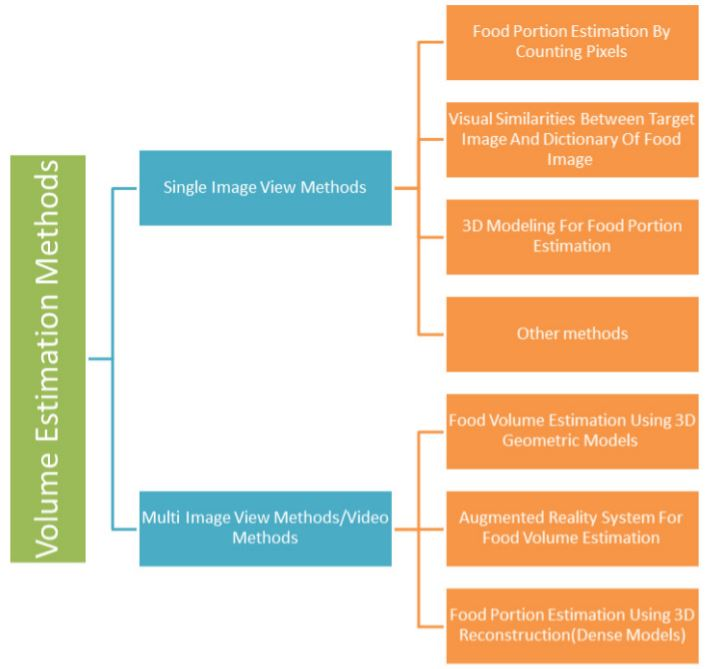
\includegraphics[width=0.7\textwidth]{2/imagen2/3FIGURA3PAPER1.JPG}
			\caption{categorizacion de estimacion de volumen}
			\label{fig6}
		\end{center}
		
	\end{figure}

\thinspace

El método de vista de imagen única para estimar el volumen de alimentos requiere solo de una imagen, por lo que son más fáciles de usar, pero son menos precisos. En cambio el de vista de múltiples imágenes, es más preciso, pero más complicado de usar debido a las múltiples imágenes desde diferentes ángulos que usan para proporcionar mejores resultados. 
\thinspace

\textbf{Resultados y conclusiones}

\thinspace
Las técnicas visuales profundas muestran un mayor rendimiento en la clasificación de alimentos, en el caso de la estimación de volúmenes de alimentos es posible calcular de manera precisa el tamaño de las porciones. Para el caso de reconocimiento de alimentos se usaron procesos como la adquisición, extracción, selección de características relevantes y la elección de la técnica de clasificación, como en la figura \ref{fig7}

\begin{figure}[h]
		\begin{center}
			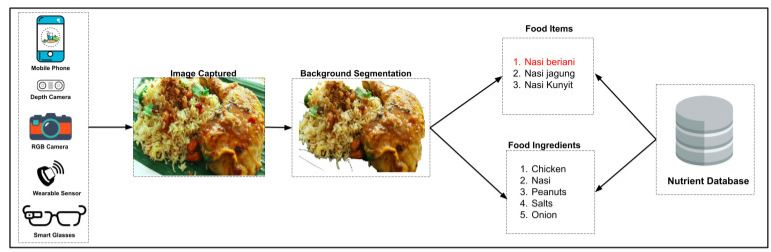
\includegraphics[width=0.7\textwidth]{2/imagen2/5FIGURA5PAPER1.JPG}
			\caption{Flujo del sistema}
			\label{fig7}
		\end{center}
		
	\end{figure}

\thinspace

 Los artículos muestran que el 38.1\% de los conjuntos de datos son genéricos, y el 46.2\% implementan CNN para el reconocimiento de alimentos. Para estimar el volumen de alimento se recomienda usar el de vista múltiple, en la figura \ref{fig8} se muestra la comparación de métodos de vista múltiple para la estimación del volumen de alimentos. 
 
\begin{figure}[h]
		\begin{center}
			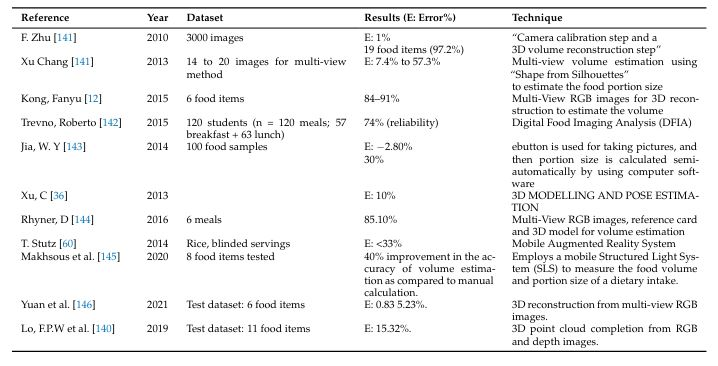
\includegraphics[width=0.7\textwidth]{2/imagen2/4FIGURA4PAPER1.JPG}
	        \caption{Comparación de métodos multivista para la estimación del volumen}
			\label{fig8}
		\end{center}
		
	\end{figure}

\thinspace

\subsection{Paper 3: DeepFood: Food Image Analysis and Dietary Assessment via Deep Model (2020)}

Los autores son Jiang, L., Bojia Q., Liu, X., Huang, C. \& Lin, K de la Facultad de Ciencias de la Computación, Universidad McGill, Montreal, Canadá, \parencite{jiang2020deepfood}

\textbf{Resumen}

\thinspace
Los avances en las herramientas de evaluación dietética y análisis nutricional mejoran la salud alimenticia, hay maneras de comprender los hábitos alimentarios diarios, explorando patrones nutricionales y promoviendo una dieta saludable. En este estudio, se muestra un sistema de evaluación dietética y reconocimiento de alimentos por aprendizaje profundo diseñado para analizar alimentos a partir de imágenes de comidas captadas por teléfonos inteligentes, por medio de tres pasos. 

Primero, se detectan las regiones candidatas en las imágenes utilizando una red de propuesta de región (RPN) derivada del modelo Faster R-CNN, segundo, estas regiones se mapean en características y se clasifican en diferentes categorías utilizando una red neuronal convolucional profunda (CNN), lo que permite su identificación en las imágenes originales. Finalmente, el sistema analiza el contenido nutricional de los alimentos reconocidos, calculando parámetros como calorías, grasas, carbohidratos y proteínas para después generar un informe de evaluación dietética. Se utilizaron dos conjuntos de datos de imágenes de alimentos conocidos (UEC-FOOD100 y UEC-FOOD256), además de introducir un nuevo conjunto de datos basado en FOOD101. Este modelo muestra una alta precisión en el reconocimiento de alimentos y genera informes de evaluación, brindando a los usuarios información valiosa sobre hábitos alimentarios saludables para una mejor salud y bienestar corporal a través de elecciones dietéticas informadas.
\thinspace

\textbf{Metodología}

\thinspace
El sistema basado en aprendizaje profundo en la detección de alimentos y se analiza los componentes nutricionales de cada imagen de comida, figura \ref{fig9}, el cual consta de tres pasos:

• Primero se extrae las regiones de interés (ROI) aplicando la red de propuesta de región derivada del modelo Faster R-CNN, con ello se separa los alimentos del fondo y mejora la eficiencia del modelo de detección.

• Segundo, se aplica una red neuronal convolucional (CNN) y se clasifica en diferentes categorías de alimentos, también se utiliza un módulo de regresión para localizar las coordenadas de los alimentos en la imagen.

• Tercero, se utilizan herramientas de evaluación dietética para el análisis de la nutrición de los alimentos y generar un informe de salud.

\begin{figure}[h]
		\begin{center}
			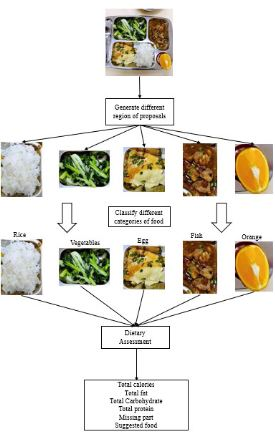
\includegraphics[width=0.5\textwidth]{2/imagen2/9FIGURA9PAPER3.JPG}
	        \caption{Reconocimiento de alimentos y análisis nutricional.}
			\label{fig9}
		\end{center}
		
	\end{figure}

\thinspace
Para la detección de alimentos, se extraen los alimentos del fondo de las imágenes y se aplica Faster R-CNN para detectar las regiones relacionadas con los alimentos. 
Para la clasificación de los alimentos, se usó la regresión del cuadro delimitador, figura \ref{fig10},  donde se ajusta el cuadro delimitador inicial para que sus coordenadas coincidan con la verdad fundamental.

\begin{figure}[h]
		\begin{center}
			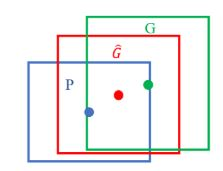
\includegraphics[width=0.2\textwidth]{2/imagen2/10FIGURA10PAPER3.JPG}
	        \caption{Regresión del Bounding box}
			\label{fig10}
		\end{center}
		
	\end{figure}

\thinspace
Para las métricas de evaluación se usó la precisión promedio media (mAP) para evaluar el modelo de detección, seguido de dos modelos: clasificación y regresión. La clasificación determina si un objeto existe en la imagen y la regresión determina la ubicación del objeto.

\thinspace
\textbf{Resultados y conclusiones}

\thinspace
En la figura \ref{fig11} se muestran los resultados en el conjunto de datos UEC-FOOD100, donde el conjunto 1 es el experimento que utilizó todas las clases de alimentos, el conjunto 2, prueba 53 clases y el conjunto 3,con 11 clases.

\begin{figure}[h]
		\begin{center}
			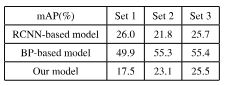
\includegraphics[width=0.5\textwidth]{2/imagen2/11FIGURA11PAPER3.JPG}
	        \caption{Los resultados en el conjunto de datos UEC-FOOD100}
			\label{fig11}
		\end{center}
		
	\end{figure}

\thinspace
En la figura \ref{fig12} se muestran los resultados en el conjunto de datos UEC-FOOD256, donde la categoría 1 es el experimento que prueba con todas las clases de alimentos, la categoría 2,con 132 clases y la categoría 3, con 21 clases.

\begin{figure}[h]
		\begin{center}
			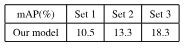
\includegraphics[width=0.5\textwidth]{2/imagen2/12FIGURA12PAPER3.JPG}
	        \caption{Los resultados en el conjunto de datos UEC-FOOD256}
			\label{fig12}
		\end{center}
		
	\end{figure}

\thinspace
Los resultados en FOOD20 con bbx se muestran en la figura \ref{fig13}.

\begin{figure}[h]
		\begin{center}
			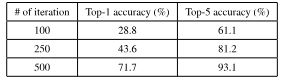
\includegraphics[width=0.5\textwidth]{2/imagen2/13FIGURA13PAPER3.JPG}
	        \caption{Los resultados en el conjunto de datos FOOD20}
			\label{fig13}
		\end{center}
		
	\end{figure}

\thinspace
Se espera mejorar la precisión de la detección, reducir el tiempo de procesamiento, y como trabajos futuros tener la predicción del peso y crear una calculadora de dieta.

\subsection{Paper 4: Image-Based Food Classification and Volume Estimation for Dietary Assessment: A Review (2020)}

Los autores son  Wen, F., Sun Y., Qiu J. \& Lo, B.. del Imperial College London, Londres, Reino Unido, publicado en el año 2020. \parencite{lo2020image}

\textbf{Resumen}

\thinspace
Existen varios métodos de evaluación dietética basados en imágenes. Este artículo compara modelos de reconocimiento de alimentos y la estimación de volumen/peso con respecto a la velocidad, precisión, eficiencia y limitaciones del procesamiento. También analiza la eficacia de métodos en el aprendizaje profundo para la evaluación dietética que combinan diferentes enfoques.

\textbf{Metodología}

\thinspace
Se usaron tres métodos para evaluar la ingesta dietética. El primero es el método de datos donde se localiza alimentos en imágenes y/o videos para reducir el almacenamiento de memoria. El segundo es el método de reconocimiento automático de alimentos, que ayuda a identificar los alimentos consumidos por los usuarios. El tercero es el método de estimación del volumen de alimentos, donde se utilizan técnicas para medir las porciones de alimento, como se muestra en la figura \ref{fig14}.

\begin{figure}[h]
		\begin{center}
			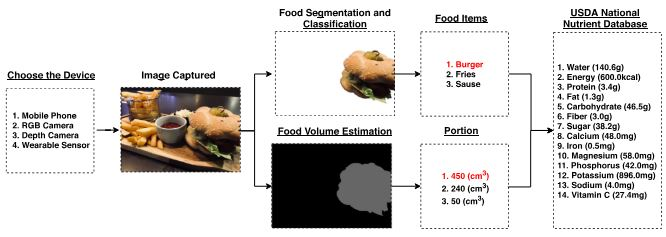
\includegraphics[width=0.5\textwidth]{2/imagen2/15FIGURA15PAPER4.JPG}
	        \caption{Diagrama del sistema para la evaluación dietética}
			\label{fig14}
		\end{center}
		
	\end{figure}

Para el reconocimiento de características de alimentos de timan en cuenta el el color, la forma y la textura, por ello hay dos enfoque principales: el reconocimiento de imágenes convencional con funciones diseñadas manualmente y el reconocimiento de imágenes de un extremo a otro con aprendizaje profundo.

En el caso del reconocimiento de imágenes convencional se usan técnicas de extracción de características como SIFT, HOG y LBP para extraer datos visuales. Para la calificación se utilizan técnicas como SVM lineal, ANN y Random Forests. Los sistemas en tiempo real utilizan técnicas de codificación como Fisher Vector para acelerar el reconocimiento. Para el aprendizaje profundo se usa las redes neuronales convolucionales (CNN)  y para la estimación de volumen de alimentos de usaron metodos como: Stereo-based Approach, Model-based, Depth Camera-based, Perspective Transformation y Deep learning, como se muestra en la figura \ref{fig15}

\begin{figure}[h]
		\begin{center}
			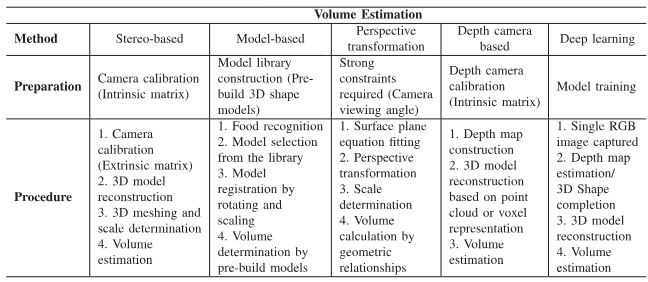
\includegraphics[width=0.5\textwidth]{2/imagen2/14FIGURA14PAPER4.JPG}
	        \caption{ Modelos para la estimación de volumen}
			\label{fig15}
		\end{center}
		
	\end{figure}

\textbf{Resultados y conclusiones}

\thinspace
La figura \ref{fig16} muestra la implementación del stereo-based volume estimation.

\begin{figure}[h]
		\begin{center}
			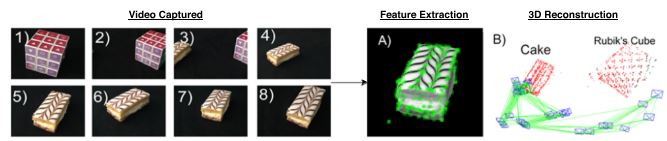
\includegraphics[width=0.5\textwidth]{2/imagen2/16FIGURA16PAPER4.JPG}
	        \caption{ implementación de la stereo-based volume estimation}
			\label{fig16}
		\end{center}
		
	\end{figure}


Los 12 mejores enfoques de aprendizaje profundo sobre clasificación de alimentos se muestran en la figura \ref{fig17}.

\begin{figure}[h]
		\begin{center}
			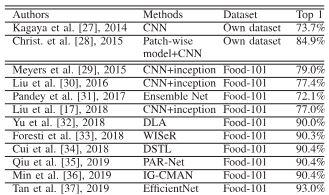
\includegraphics[width=0.5\textwidth]{2/imagen2/17FIGURA17PAPER4.JPG}
	        \caption{  Enfoques de aprendizaje profundo, TOP 12}
			\label{fig17}
		\end{center}
		
	\end{figure}

 En el reconocimiento de alimentos mediante imágenes se ha demostrado que las redes neuronales profundas superan a los enfoques tradicionales basados en características manuales. Sin embargo, persisten desafíos en la estimación de la ingesta nutricional debido al tamaño de las porciones y requieren de múltiples capturas de imágenes desde diferentes ángulos.

 \subsection{Paper 5: Deep Neural Networks for Image-Based Dietary Assessment (2021)} 

Koroušić, B. \&  Mezgec, S. del Departamento de Sistemas Informáticos Ljubljana, Eslovenia, \parencite{mezgec2021deep}.

\textbf{Resumen}

\thinspace
Con la tecnología, hoy en día, se puede registrar la ingesta con solo tomar una foto desde la cámara celular. Este artículo habla sobre el reconocimiento de alimentos en imágenes por medio de las redes neuronales profundas, utilizando la arquitectura de Nutrinet la cual es una modificación de la arquitectura AlexNet14. Aunque Nutrinet se limita a una salida de imagen de alimento,esta utiliza segmentación de imágenes ya que identifica la cantidad de alimentos y bebidas en una imagen. Los principales métodos de segmentación en este artículo son las redes totalmente convolucionales (FCN) y el otro en redes residuales profundas (ResNet). Anteriormente se ha usado extractores de características definidas manualmente pero solo han tenido precisión entre el 10\% - 40\% considerándose bajo por su apariencia variable de cada presentación de comida. Las redes neuronales convolucionales profundas (DCNN) son las más populares para el reconocimiento de imágenes de alimentos. Las capas convolucionales contienen filtros que aprenden y que responden a ciertas características de los datos de entrada, mientras que las capas completamente conectadas componen datos de salida de otras capas para obtener conocimientos de nivel superior a partir de ellos. 

\textbf{Metodología}

\thinspace
Se utilizó la arquitectura NutriNet,figura \ref{fig18}. Para la segmentación de imágenes se tomaron dos arquitecturas: las variaciones de las redes totalmente convolucionales (FCN-32, FCN-16 y FCN-8s15 ) y las redes residuales profundas (ResNet), como principales tomo AlexNet14, GoogLeNet y ResNet. Para el procesamiento de datos se tomó el Food Recognition Challenge y el método de Hybrid Task Cascade con ResNet-10116, también se utilizó otras redes troncales, pero se tomó la ResNet-101 como la más adecuada. Entre los parámetros de entrenamiento para tener valores óptimos se eligió el solucionador, que determina la precisión en la clasificación; la tasa de aprendizaje, donde se define la velocidad con la cambia el parámetro de la red neuronal. 

\begin{figure}[h]
		\begin{center}
			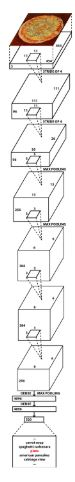
\includegraphics[width=0.05\textwidth]{2/imagen2/20FIGURA20PAPER4.JPG}
	        \caption{ Arquitectura de red neuronal profunda NutriNet}
			\label{fig18}
		\end{center}
		
	\end{figure}
 
\textbf{Resultados y conclusiones}

\thinspace
Los modelos AlexNet se entrenaron utilizando un tamaño de lote de 256 imágenes y una tasa de aprendizaje base de 0,02; NutriNet utilizó un tamaño de lote de 128 imágenes y una tasa de 0,01; GoogLeNet 64 imágenes y una tasa de 0,005; y ResNet 16 imágenes y una tasa de 0,00125, figura \ref{fig19}

\begin{figure}[h]
		\begin{center}
			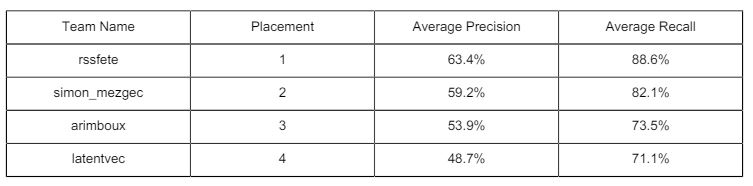
\includegraphics[width=0.7\textwidth]{2/imagen2/21FIGURA21PAPER4.JPG}
	        \caption{Reconocimiento de Alimentos}
			\label{fig19}
		\end{center}
		
	\end{figure}

Para entrenar el modelo de segmentación de imágenes de alimentos falsos del FCN-8, utilizamos Adam55. La precisión final del modelo FCN-8 entrenado fue del 92,18\%. la figura \ref{fig20} muestra, imágenes de alimentos falsos (una de cada uno de los subconjuntos de entrenamiento, validación y prueba), junto con las correspondientes etiquetas de predicción del modelo y de verdad sobre el terreno.

\begin{figure}[h]
		\begin{center}
			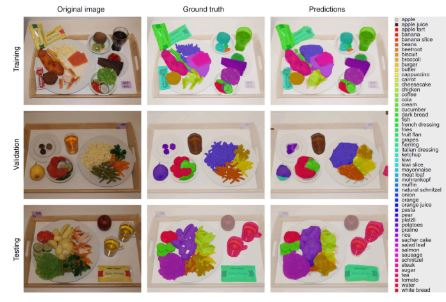
\includegraphics[width=0.5\textwidth]{2/imagen2/22FIGURA22PAPER4.JPG}
	        \caption{ Imágenes del conjunto de datos de imágenes de alimentos falsos}
			\label{fig20}
		\end{center}
		
	\end{figure}

\section{Bases Teóricas}

\subsection{Inteligencia Artificial}

Existen diferentes definiciones que complementan a la definición de la inteligencia artificial (IA),la Asociación para el Progreso de la Dirección (\parencite{apda}) lo explica como un campo en la ciencia e ingeniería que se encarga de la comprensión desde el punto de vista informático, lo cual lo conocen como un comportamiento inteligente. 

La inteligencia artificial es representada por un conjunto de tecnologías que buscan que las computadoras puedan comportarse como “humanos” o asemejarse a ellos desarrollando capacidades como ver, pensar, hablar, escribir; también que ayuden a reducir los tiempos de tareas, ofrezcan recomendaciones y puedan analizar datos en grandes o pequeñas cantidades, lo cual es explicado a más detalle en \parencite{googlee}. 

Algunas situaciones técnicas dadas por \cite{Rouhiainen}, muestran donde la inteligencia artificial puede ser aplicada como, por ejemplo, en el reconocimiento, clasificación y etiquetado de imágenes, eficiencia en las estrategias comerciales, procesamientos escalables de datos, predicción, detección de objetos, ciberseguridad. La inteligencia artificial funciona a través de algoritmos que toman decisiones basadas en objetivos o tareas ya establecidas, con ello pueden aprovechar al máximo la información disponible. 


\subsection{Aprendizaje Automático}

Según \cite{soria} la definición del aprendizaje automático o aprendizaje de maquina es la optimización del criterio de rendimiento que utiliza los datos de ejemplo y las experiencias anteriores, con ello expresa una de las características técnicas del concepto. En una diferenciación frente a las otras áreas de la Inteligencia Artificial, es la tarea dada a una computadora que aprende y las experiencias que puede rescatar de dichas tareas a medida que se va desarrollando logrando así mejorar su rendimiento. 
Machine learning o aprendizaje automático es uno de los enfoques más conocido en el área de la inteligencia artificial. Para \cite{Rouhiainen}, el aprendizaje automático utiliza algoritmos que le ayudan a aprender los patrones de datos. 
Existen tres principales tipos de aprendizaje automático, los supervisados, que están basados en tareas; el aprendizaje no supervisados, que está basado en datos y el aprendizaje por refuerzo, que aprende reaccionando a su entorno. 
La atención al cliente, seguridad, marketing digital, phishing u otros fraudes son algunos de los casos de usos propuestos por Google Cloud

\subsection{Aprendizaje Profundo}

Microsoft define al aprendizaje profundo o deep learning (DL) como un tipo de aprendizaje automático el cual usa las redes neuronales artificiales para permitir que las maquinas puedan aprender y logren tomar decisiones basadas en datos los cuales pues estar no estructurados. Según \cite{Rouhiainen}, el aprendizaje profundo es el más escalable en toda la inteligencia artificial, este sub campo resuelve problemas complejos en grandes cantidades de datos.  

\cite{xin2018machine} expica que una de las mayores ventajas del uso del aprendizaje profundo es su alto rendimiento en una variedad de campos complejos que cuentan con grandes cantidades de data, las cuales pueden ser aplicados en los campos de salud, seguridad y otros. 


\subsection{Redes Neuronales Convolucionales (CNN)}

Un modelo de red neuronal convolucional o conocido en inglés como convolutional neural networks (CNN) puede aprender desde los datos presentes sin alguna extracción de características \parencite{xin2018machine}

Para Google Cloud las redes neuronales convolucionales suelen ser usadas en el reconocimiento de imágenes y emplean diversas capas que separan en partes la imagen dada antes de unirla nuevamente. Con ello se encuentran características comunes como los colores, bordes, tamaño y otras características más complejas. Cada nodo presentado en la red neuronal tiene un peso y está conectado al siguiente nodo, este logra activarse si la salida del nodo es mayor a un especifico umbral de la red, caso contrario este no logra pasar ningún dato a la siguiente capa, tal como lo detalla IBM.



\subsection{Visión por Computadora}

Visón por computadora o visión artificial permite a las computadoras obtener información de imágenes, videos u otras entradas de origen visual para tomar acciones como reconocer e identificar cierta cantidad de ellas (IBM).

\parencite{bohr2021inteligencia} mencionan que se tiene una buena comprensión de las imágenes y videos; y aunque antes tenía pocas aplicaciones debido a algunas capacidades limitadas en los enfoques de la inteligencia artificial, con el paso del tiempo ha logrado brindar gran ayuda a diferentes campos gracias a las redes convencionales. La mayoría de casos de usos que usan la visión por computadora son destinadas a resolver una tarea 


\subsection{Síndrome Metabólico}

Para \parencite{ramos2022sindrome}, el síndrome metabólico o síndrome X es una situación médica que abarca un conjunto de alteraciones cardiometabólicas como la hipertensión, la obesidad, la resistencia a la insulina.

Como se mustra en la figura \ref{fig24}, las bases para el diagnóstico del síndrome metabólico fueron propuestas por varias organizaciones en diferentes años, entre las principales se encuentran: la Organización Mundial de la Salud (OMC), European Group for the Study of Insulin Resistence (EGIR), el Panel III de Tratamiento de Adultos del Programa Nacional de Educación sobre el Colesterol (NCEP/ATPIII), la Asociación Estadounidense de Endocrinólogos Clínicos (AACE/ADA), la Fundación Internacional de Diabetes (IDF), la Asociación Estadounidense del Corazón e Instituto Nacional del Corazón, los Pulmones y la Sangre (AHA/NHLBI).

\thinspace

\begin{figure}[h]
		\begin{center}
			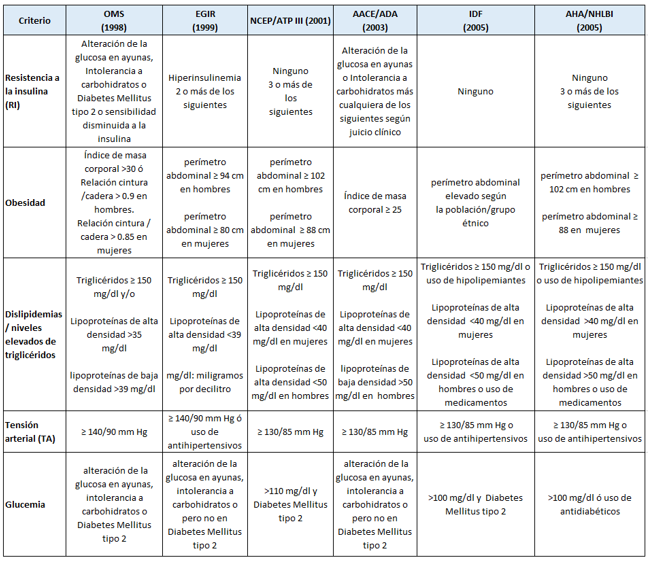
\includegraphics[width=1\textwidth]{2/imagen2/oms.PNG}
	        \caption{Revista médica de Guadalajara }
			\label{fig24}
		\end{center}
		
	\end{figure}

\thinspace


\subsection{Valor nutricional}

El valor nutricional en un alimento comprende el valor energético y sus nutrientes tales como las proteínas, las grasas, los carbohidratos, las fibras, los azucares, el sodio, las vitaminas, los minerales, entre otros \parencite{nestle}. Este valor es dado por su composición química y depende se otros factores como su almacenamiento, fertilización, esterilización, estado de madurez. 

Según la organización de las naciones unidas para la alimentación y la agricultura o FAO, el contenido de los nutrientes es cado cuando se pasan los 100 gramos de proporción comestible. Un único alimento puede variar su contenido dependiendo la condición en la que se encuentra como, por ejemplo, puede estar crudo, cocido, hervido o frito.


\section{Marco Conceptual}

\subsection{Matriz de Confusión}

En \parencite{tahir2021comprehensive} se menciona que las matrices de confusión son usadas para ver en general el rendimiento de un modelo de clasificacion en el aprendizaje automatico

Una matriz de confusión muestra, definido por Google Cloud, es la frecuencia de un resultado predicho en un modelo.El objetivo de la matriz de confusión es que se logre comprender donde el modelo "confunde" resultados bilateral 

Los cuatro resultados pueden ser:

Verdadero Positivo (TP): Predicho Verdadero y Verdadero en realidad.
\thinspace

Verdadero Negativo (TN): Predicho Falso y Falso en realidad.
\thinspace

Falso Positivo (FP): Predicción de verdadero y falso en la realidad.
\thinspace

Falso Negativo (FN): Predicción de falso y verdadero en la realidad.

\subsection{Accuracy o Exactitud}

Para \cite{tahir2021comprehensive} parencite{tahir2021comprehensive}, la exactitud de un modelo sirve para predecir de manera efectiva si clases o un modelo general.

Esta medida muestra la cercanía de las predicciones de un modelo de los valores reales. El resultado es un porcentaje que se clasifica correctamente. También, la exactitud es usada cuando hay dos clases con tamaños similares. En el caso de la tasa de error, sirve para definir con que frecuencia hay errores, \cite{datasour} 

\subsection{F1 Score}

La puntuación F1 es la precisión o proporción de VF entre los positivos predichos; y la exhaustividad es la proporción de VF entre los positivos reales. Tambien, \cite{tahir2021comprehensive} menciona que la puntuación F1 se toma como la media armónica de la puntuación y precisión.


\subsection{Handcrafted Features}

Las características hechas a mano son datos diseñados manualmente basándose en el problema, con el fin de mejorar el rendimiento de un modelo de aprendizaje automático. Estas características se crean para resaltar patrones relevantes en los datos. Para el contexto en el reconocimiento de imágenes, las características pueden  tener variaciones en su forma y color, lo que ayuda a diferenciar entre distintos tipos de alimentos, \cite{tahir2021comprehensive}.

Los métodos son:

1. Características de la forma: PHOG, GIST.
\thinspace

2. Funciones locales: SIFT, SURF, CSFIT, descriptor Daisy.
\thinspace

3. Características de color: HOG, histograma de color, histogramas RGB
\thinspace

4. Características de textura: LBP, LPQ, LCP, GBP, textons, PRICoLBP
\thinspace

\subsection{Multi-stage architecture} 
Es parte de las arquitecturas de evaluación dietética basada en la visión (VBDA), descrito en el artículo \textit{A review on vision-based analysis for automatic dietary assessment}, \cite{wang2022review}. El cual consiste de tres etapas: análisis de imágenes, estimación de porciones y derivación de nutrientes. Donde las primeras dos etapas dependen de los algoritmos de Inteligencia artificial y de la data de alimentos , mientras que la tercera etapa, de la data de composición nutricional.

\begin{itemize}
    \item Fase 1 : Análisis de imágenes, donde se reconoce, detecta y segmenta los alimentos.
    \item Fase 2 : Estimación de porciones, donde se estima con precisión el contenido de nutrientes de los alimento desde una imagen
    \item Fase 3 : Derivación de nutrientes, donde se realiza la conversión de alimentos a información nutricional significativa.
    
\end{itemize}


\chapter{METODOLOGÍA DE LA INVESTIGACIÓN}

\section{Diseño de la investigación}

\subsection{Tipo de la investigación}

El tipo de investigacion para este presente trabajo es experimental, puesto que se  analizan imágenes y se lleva a cabo un diseño de implementación y evaluación de una aplicacion por vision por computadora que monitorea el consumo de carbohidratos de los alimentos de estudiantes universitarios. También se realizarán pruebas para medir la efectividad de la aplicación y notar si es de utilidad para la prevensión del síndrome meabólico.

\subsection{Enfoque de la investigacion}

El enfoque para este presente trabajo es cuantitativo, debido a que se realizará una representación de pixeles por cada imagen  presentada en la base de datos, seguido de un redimensionamiento y representación numérica. También los instrumentos a usar se harán por aproximaciones que serán medidas, tales como el uso del precisión y sensibilidad. 

\subsection{Poblacion}

La población es representada por las imágenes de alimentos que son consumidos por estudiantes universitarios, como platos de comida peruanos e internacionales, imágenes de postres simples y comidas rápidas extraídas de la plataforma Kaggle. Las imágenes deben estar en buena calidad y no tener ruido, es decir, no estar cargadas de otros objetos que no sean los alimentos requeridos, tampoco deben de presentarse borrosas. 

\subsection{Muestra}

La muestra es representada por mas de mil imagenes de platos de comida, puede ser del tipo platos de comidas peruanas e internacionales, postres y comidas rápidas, 

\subsection{Operacionalización de Variables}

En la Tabla \ref{3:table1} se presenta la operacionalización de variables para la investigación.

\begin{table}[h!]
  \centering
  \caption{Variables e Indicadores}
  \label{3:table1}
  \begin{tabular}{|p{0.5\linewidth}|p{0.4\linewidth}|}
    \hline
    \textbf{Variables} & \textbf{Indicadores} \\
    \hline
    Dependiente: Prevención del síndrome metabólico en estudiantes universitarios.
    
    \thinspace
    
    Independiente: Aplicación para monitorear carbohidratos aplicando visión por computadora.
    & \vspace{1mm} Precisión (Accuracy): $\frac{TP + TN}{TP + TN + FP + FN}$ \\
    & Recall (Sensibilidad): $\frac{TP}{TP + FN}$ \\
    & F1-score: $2 \times \frac{\text{Precision} \times \text{Recall}}{\text{Precision} + \text{Recall}}$ \\
    & Área bajo la curva ROC \\
    \hline
  \end{tabular}
\end{table}

El trabajo busca prevenir el síndrome metabolico  a través de una aplicacion de visión por computadora que monitorea el consumo de carbohidratos. 
%\include{4/desarrollo}
%\include{5/resultados}
%\include{6/conclusion}
%%Anexos
\appendix
\renewcommand{\appendixname}{Anexos}
\renewcommand{\appendixtocname}{Anexos}
\renewcommand{\appendixpagename}{Anexos}
\clearpage
\addappheadtotoc
\appendixpage
\chapter{Anexo I: Árbol del problema}

\begin{figure}[h]
		\begin{center}
			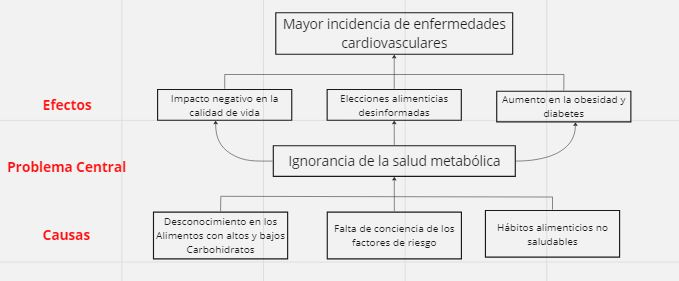
\includegraphics[width=1.1\textwidth]{1/figures/arbol de problems.JPG}
			\caption{Prueba de Figura}
			\label{fig1}
		\end{center}
		
	\end{figure}

\chapter{Anexo II: Árbol del objetivos}

\begin{figure}[h]
		\begin{center}
			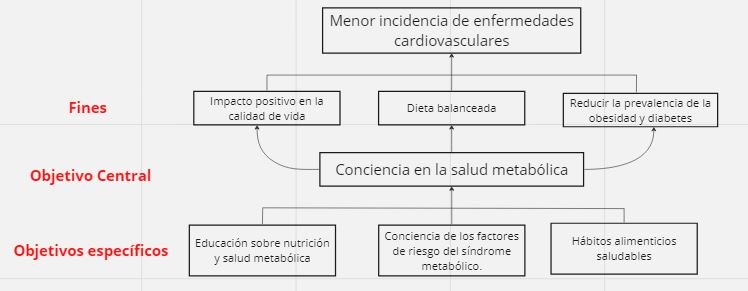
\includegraphics[width=1.1\textwidth]{1/figures/arbol de objetivos.JPG}
			\caption{Prueba de Figura}
			\label{fig1}
		\end{center}
		
	\end{figure}

\chapter{Anexo III: Matriz de Consistencia}

\begin{table}[h!]
	\centering
	\small
	\begin{tabular}{ |m{5cm}|m{5cm}|m{5cm}| }
		\hline
		\rowcolor{bluejean}
		\Centering \color{white}{PROBLEMAS}& \Centering \color{white}{OBJETIVOS}& \Centering \color{white}{HIPÓTESIS}\\
		\hline
		\rowcolor{turq}
		\Centering Problema General& \Centering Objetivo General & \Centering Hipotesis General \\
		\hline
  
        \ProblemaGeneral & 
        \ObjetivoGeneral  & 
        \HipotesisGeneral \\
        \hline
		
        \rowcolor{turq}
		\Centering Problemas Específicos& \Centering Objetivos Específicos & \Centering Hipotesis Específicas \\
		\hline
  
		{\Pbone} & {\Objone} & {\Hone} \\
		\hline
		{\Pbtwo} & {\Objtwo} & {\Htwo} \\
		\hline
		{\Pbthree} & {\Objthree} & {\Hthree} \\
		\hline
            {\Pbfour} & {\Objfour} & {\Hfour} \\
		\hline
	\end{tabular}
	\caption{Matriz de consistencia. Fuente: Elaboración propia}
	\label{1:table}
\end{table}







% %%Bibliografia
%\bibliographystyle{apalike} % Title is link if provided
%\renewcommand{\bibname}{BIBLIOGRAFÍA} % changes the header; default: Bibliography

\printbibliography[heading=bibintoc,title={BIBLIOGRAFÍA}]
%\bibliography{biblio/references} % adjust this to fit your BibTex file
\end{document}

